\chapter{Zeichnungstypen von Nodes}
\label{ch:items/node-drawtypes}

Die Art, wie ein Node gezeichnet wird, heißt
\emph{Zeichnungstyp\index{zeichnungstyp@Zeichnungstyp}}
(\emph{drawtype}). Es gibt viele davon. Das Verhalten eines
Zeichnungstyps steuerst du über Eigenschaften in der Definition des
Node-Typs. Diese Eigenschaften gelten für alle Instanzen dieses Nodes;
manche lassen sich aber über \texttt{param2} auch je Node steuern.

Im vorigen Kapitel wurden Nodes und Items eingeführt, eine vollständige
Definition eines Nodes fehlte aber noch. Die Luanti-Welt ist ein
3D-Gitter aus Positionen. Jede Position heißt Node und besteht aus dem
Node-Typ (Name) und zwei Parametern (\texttt{param1} und
\texttt{param2}). Der Name der Funktion
\texttt{core.\allowbreak{}register\_\allowbreak{}node}\index{core@\texttt{core}!register_node@\texttt{core.\allowbreak{}register\_\allowbreak{}node}}
ist etwas irreführend: Sie registriert nicht wirklich einen Node,
sondern einen neuen \emph{Typ} von Node.

Die Node-Parameter steuern, wie ein einzelner Node dargestellt wird.
\texttt{param1} speichert die Beleuchtung eines Nodes; die Bedeutung von
\texttt{param2} hängt von der Eigenschaft \texttt{paramtype2} der
Node-Typ-Definition ab.

\section{Würfelförmige Nodes: normal und
allfaces}\label{wuxfcrfelfuxf6rmige-nodes-normal-und-allfaces}

\begin{figure}
\centering
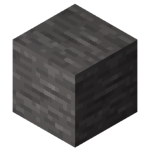
\includegraphics[width=4cm,height=\textheight,keepaspectratio,alt={Zeichnungstyp normal}]{bilder/drawtype_normal.png}
\caption{Zeichnungstyp normal}
\end{figure}

Der Zeichnungstyp \texttt{normal} wird typischerweise für würfelförmige
Nodes verwendet. Liegt eine Seite eines normalen Nodes an einer festen
Seite an, wird sie nicht gezeichnet. Das bringt einen großen
Leistungsgewinn.

Der Zeichnungstyp \texttt{allfaces} zeichnet dagegen auch die
Innenseite, wenn sie an einem festen Node anliegt. Das eignet sich für
Nodes mit teilweise transparenten Seiten, etwa Blätter. Mit
\texttt{allfaces\_\allowbreak{}optional} können Benutzer das langsamere
Zeichnen abschalten; der Node verhält sich dann wie ein normaler Node.

\begin{Shaded}
\begin{Highlighting}[]
\VariableTok{core}\OperatorTok{.}\NormalTok{register\_node}\OperatorTok{(}\StringTok{"mymod:diamond"}\OperatorTok{,} \OperatorTok{\{}
    \VariableTok{description} \OperatorTok{=} \StringTok{"Alien{-}Diamant"}\OperatorTok{,}
    \VariableTok{tiles} \OperatorTok{=} \OperatorTok{\{} \StringTok{"mymod\_diamond.png"} \OperatorTok{\},}
    \VariableTok{groups} \OperatorTok{=} \OperatorTok{\{} \VariableTok{cracky} \OperatorTok{=} \DecValTok{3} \OperatorTok{\},}
\OperatorTok{\})}

\VariableTok{core}\OperatorTok{.}\NormalTok{register\_node}\OperatorTok{(}\StringTok{"default:leaves"}\OperatorTok{,} \OperatorTok{\{}
    \VariableTok{description} \OperatorTok{=} \StringTok{"Blätter"}\OperatorTok{,}
    \VariableTok{drawtype} \OperatorTok{=} \StringTok{"allfaces\_optional"}\OperatorTok{,}
    \VariableTok{tiles} \OperatorTok{=} \OperatorTok{\{} \StringTok{"default\_leaves.png"} \OperatorTok{\},}
\OperatorTok{\})}
\end{Highlighting}
\end{Shaded}

Hinweis: \texttt{normal} ist der Standard-Zeichnungstyp, du musst ihn
also nicht ausdrücklich angeben.

\section{Glasartige Nodes}\label{glasartige-nodes}

Der Unterschied zwischen glasartigen (\texttt{glasslike}) und normalen
Nodes: Steht ein glasartiger Node neben einem normalen, wird die
angrenzende Seite des normalen Nodes trotzdem gezeichnet. Das ist
nützlich, weil glasartige Nodes meist transparent sind -- mit dem
Zeichnungstyp \texttt{normal} könnte man sonst durch die Welt
hindurchsehen.

\begin{figure}
\centering
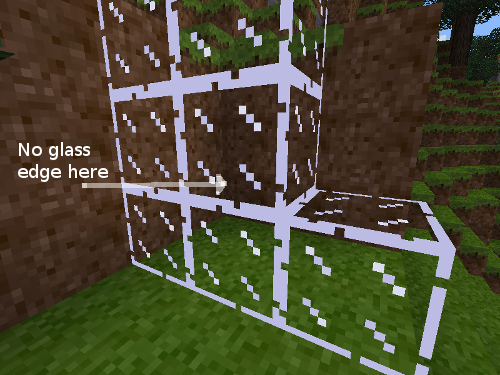
\includegraphics[width=7cm,height=\textheight,keepaspectratio,alt={Kanten bei glasslike}]{bilder/drawtype_glasslike_edges.png}
\caption{Kanten bei glasslike}
\end{figure}

\begin{Shaded}
\begin{Highlighting}[]
\VariableTok{core}\OperatorTok{.}\NormalTok{register\_node}\OperatorTok{(}\StringTok{"default:obsidian\_glass"}\OperatorTok{,} \OperatorTok{\{}
    \VariableTok{description} \OperatorTok{=} \StringTok{"Obsidianglas"}\OperatorTok{,}
    \VariableTok{drawtype} \OperatorTok{=} \StringTok{"glasslike"}\OperatorTok{,}
    \VariableTok{tiles} \OperatorTok{=} \OperatorTok{\{} \StringTok{"default\_obsidian\_glass.png"} \OperatorTok{\},}
    \VariableTok{paramtype} \OperatorTok{=} \StringTok{"light"}\OperatorTok{,}
    \VariableTok{is\_ground\_content} \OperatorTok{=} \KeywordTok{false}\OperatorTok{,}
    \VariableTok{sunlight\_propagates} \OperatorTok{=} \KeywordTok{true}\OperatorTok{,}
    \VariableTok{sounds} \OperatorTok{=} \VariableTok{default}\OperatorTok{.}\NormalTok{node\_sound\_glass\_defaults}\OperatorTok{(),}
    \VariableTok{groups} \OperatorTok{=} \OperatorTok{\{} \VariableTok{cracky} \OperatorTok{=} \DecValTok{3}\OperatorTok{,} \VariableTok{oddly\_breakable\_by\_hand} \OperatorTok{=} \DecValTok{3} \OperatorTok{\},}
\OperatorTok{\})}
\end{Highlighting}
\end{Shaded}

\subsection{glasslike\_framed}\label{glasslike_framed}

Hier läuft der Rand mit einem 3D-Effekt um die gesamte zusammenhängende
Fläche statt um jeden einzelnen Node:

\begin{figure}
\centering
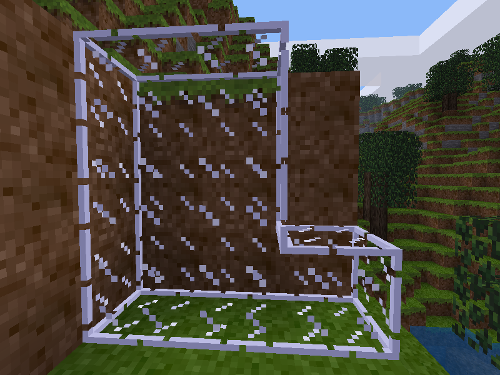
\includegraphics[width=7cm,height=\textheight,keepaspectratio,alt={Kanten bei glasslike\_framed}]{bilder/drawtype_glasslike_framed.png}
\caption{Kanten bei glasslike\_framed}
\end{figure}

Mit dem Zeichnungstyp
\texttt{glasslike\_\allowbreak{}framed\_\allowbreak{}optional} kann der
Benutzer das gerahmte Aussehen selbst \emph{einschalten}.

\begin{Shaded}
\begin{Highlighting}[]
\VariableTok{core}\OperatorTok{.}\NormalTok{register\_node}\OperatorTok{(}\StringTok{"default:glass"}\OperatorTok{,} \OperatorTok{\{}
    \VariableTok{description} \OperatorTok{=} \StringTok{"Glas"}\OperatorTok{,}
    \VariableTok{drawtype} \OperatorTok{=} \StringTok{"glasslike\_framed"}\OperatorTok{,}
    \VariableTok{tiles} \OperatorTok{=} \OperatorTok{\{}
        \StringTok{"default\_glass.png"}\OperatorTok{,}
        \StringTok{"default\_glass\_detail.png"}\OperatorTok{,}
    \OperatorTok{\},}
    \VariableTok{inventory\_image} \OperatorTok{=} \VariableTok{core}\OperatorTok{.}\NormalTok{inventorycube}\OperatorTok{(}
        \StringTok{"default\_glass.png"}
    \OperatorTok{),}
    \VariableTok{paramtype} \OperatorTok{=} \StringTok{"light"}\OperatorTok{,}
    \VariableTok{sunlight\_propagates} \OperatorTok{=} \KeywordTok{true}\OperatorTok{,} \CommentTok{{-}{-} Sonnenlicht geht durch}
    \VariableTok{groups} \OperatorTok{=} \OperatorTok{\{} \VariableTok{cracky} \OperatorTok{=} \DecValTok{3}\OperatorTok{,} \VariableTok{oddly\_breakable\_by\_hand} \OperatorTok{=} \DecValTok{3} \OperatorTok{\},}
    \VariableTok{sounds} \OperatorTok{=} \VariableTok{default}\OperatorTok{.}\NormalTok{node\_sound\_glass\_defaults}\OperatorTok{(),}
\OperatorTok{\})}
\end{Highlighting}
\end{Shaded}

\section{Luftartige Nodes}\label{luftartige-nodes}

Diese Nodes werden nicht gezeichnet und haben daher keine
Texturen.\index{textur@Textur}

\begin{Shaded}
\begin{Highlighting}[]
\VariableTok{core}\OperatorTok{.}\NormalTok{register\_node}\OperatorTok{(}\StringTok{"myair:air"}\OperatorTok{,} \OperatorTok{\{}
    \VariableTok{description} \OperatorTok{=} \StringTok{"MyAir (du Hacker, du!)"}\OperatorTok{,}
    \VariableTok{drawtype} \OperatorTok{=} \StringTok{"airlike"}\OperatorTok{,}
    \VariableTok{paramtype} \OperatorTok{=} \StringTok{"light"}\OperatorTok{,}
    \VariableTok{sunlight\_propagates} \OperatorTok{=} \KeywordTok{true}\OperatorTok{,}

    \VariableTok{walkable} \OperatorTok{=} \KeywordTok{false}\OperatorTok{,} \CommentTok{{-}{-} sonst kollidiert der Spieler}
    \VariableTok{pointable} \OperatorTok{=} \KeywordTok{false}\OperatorTok{,} \CommentTok{{-}{-} Node kann nicht ausgewählt werden}
    \VariableTok{diggable} \OperatorTok{=} \KeywordTok{false}\OperatorTok{,} \CommentTok{{-}{-} Node kann nicht abgebaut werden}
    \VariableTok{buildable\_to} \OperatorTok{=} \KeywordTok{true}\OperatorTok{,} \CommentTok{{-}{-} Nodes können diesen Node ersetzen}
    \CommentTok{{-}{-} (man kann einen Node an seine Stelle}
    \CommentTok{{-}{-} setzen, die Luft verschwindet dann)}

    \VariableTok{air\_equivalent} \OperatorTok{=} \KeywordTok{true}\OperatorTok{,}
    \VariableTok{drop} \OperatorTok{=} \StringTok{""}\OperatorTok{,}
    \VariableTok{groups} \OperatorTok{=} \OperatorTok{\{} \VariableTok{not\_in\_creative\_inventory} \OperatorTok{=} \DecValTok{1} \OperatorTok{\},}
\OperatorTok{\})}
\end{Highlighting}
\end{Shaded}

\section{Beleuchtung und Ausbreitung des
Sonnenlichts}\label{beleuchtung-und-ausbreitung-des-sonnenlichts}

Die Beleuchtung eines Nodes wird in \texttt{param1} gespeichert. Um zu
berechnen, wie eine Seite eines Nodes schattiert wird, nimmt Luanti den
Lichtwert des benachbarten Nodes. Deshalb haben feste Nodes keine
Lichtwerte -- sie blockieren das Licht ja.

Standardmäßig erlaubt ein Node-Typ nicht, Licht in seinen Instanzen zu
speichern. Bei manchen Nodes wie Glas und Luft soll Licht aber
durchgehen. Dazu müssen zwei Eigenschaften gesetzt werden:

\begin{Shaded}
\begin{Highlighting}[]
\VariableTok{paramtype} \OperatorTok{=} \StringTok{"light"}\OperatorTok{,}
\VariableTok{sunlight\_propagates} \OperatorTok{=} \KeywordTok{true}\OperatorTok{,}
\end{Highlighting}
\end{Shaded}

Die erste Zeile bedeutet, dass \texttt{param1} tatsächlich den Lichtwert
speichert. Die zweite, dass Sonnenlicht ohne Abschwächung durch den Node
hindurchgeht.

\section{Flüssige Nodes}\label{fluxfcssige-nodes}

\begin{figure}
\centering
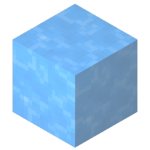
\includegraphics[width=4cm,height=\textheight,keepaspectratio,alt={Zeichnungstyp liquid}]{bilder/drawtype_liquid.png}
\caption{Zeichnungstyp liquid}
\end{figure}

Jede Flüssigkeit braucht zwei Node-Definitionen: eine für die Quelle und
eine für die fließende Flüssigkeit.

\begin{Shaded}
\begin{Highlighting}[]
\CommentTok{{-}{-} Einige Eigenschaften wurden weggelassen, weil sie über}
\CommentTok{{-}{-} dieses Kapitel hinausgehen.}
\VariableTok{core}\OperatorTok{.}\NormalTok{register\_node}\OperatorTok{(}\StringTok{"default:water\_source"}\OperatorTok{,} \OperatorTok{\{}
    \VariableTok{drawtype} \OperatorTok{=} \StringTok{"liquid"}\OperatorTok{,}
    \VariableTok{paramtype} \OperatorTok{=} \StringTok{"light"}\OperatorTok{,}

    \VariableTok{inventory\_image} \OperatorTok{=} \VariableTok{core}\OperatorTok{.}\NormalTok{inventorycube}\OperatorTok{(}
        \StringTok{"default\_water.png"}
    \OperatorTok{),}
    \CommentTok{{-}{-} \^{} nötig, damit das Inventarbild nicht animiert wird}

    \VariableTok{tiles} \OperatorTok{=} \OperatorTok{\{}
        \OperatorTok{\{}
            \VariableTok{name} \OperatorTok{=} \StringTok{"default\_water\_source\_animated.png"}\OperatorTok{,}
            \VariableTok{animation} \OperatorTok{=} \OperatorTok{\{}
                \FunctionTok{type} \OperatorTok{=} \StringTok{"vertical\_frames"}\OperatorTok{,}
                \VariableTok{aspect\_w} \OperatorTok{=} \DecValTok{16}\OperatorTok{,}
                \VariableTok{aspect\_h} \OperatorTok{=} \DecValTok{16}\OperatorTok{,}
                \VariableTok{length} \OperatorTok{=} \DecValTok{2.0}\OperatorTok{,}
            \OperatorTok{\},}
        \OperatorTok{\},}
    \OperatorTok{\},}

    \VariableTok{special\_tiles} \OperatorTok{=} \OperatorTok{\{}
        \CommentTok{{-}{-} Wasserquellen neuen Typs (kaum genutzt)}
        \OperatorTok{\{}
            \VariableTok{name} \OperatorTok{=} \StringTok{"default\_water\_source\_animated.png"}\OperatorTok{,}
            \VariableTok{animation} \OperatorTok{=} \OperatorTok{\{}
                \FunctionTok{type} \OperatorTok{=} \StringTok{"vertical\_frames"}\OperatorTok{,}
                \VariableTok{aspect\_w} \OperatorTok{=} \DecValTok{16}\OperatorTok{,}
                \VariableTok{aspect\_h} \OperatorTok{=} \DecValTok{16}\OperatorTok{,}
                \VariableTok{length} \OperatorTok{=} \DecValTok{2.0}\OperatorTok{,}
            \OperatorTok{\},}
            \VariableTok{backface\_culling} \OperatorTok{=} \KeywordTok{false}\OperatorTok{,}
        \OperatorTok{\},}
    \OperatorTok{\},}

    \CommentTok{{-}{-}}
    \CommentTok{{-}{-} Verhalten}
    \CommentTok{{-}{-}}
    \VariableTok{walkable} \OperatorTok{=} \KeywordTok{false}\OperatorTok{,} \CommentTok{{-}{-} Spieler fällt hindurch}
    \VariableTok{pointable} \OperatorTok{=} \KeywordTok{false}\OperatorTok{,} \CommentTok{{-}{-} Spieler kann es nicht auswählen}
    \VariableTok{diggable} \OperatorTok{=} \KeywordTok{false}\OperatorTok{,} \CommentTok{{-}{-} Spieler kann es nicht abbauen}
    \VariableTok{buildable\_to} \OperatorTok{=} \KeywordTok{true}\OperatorTok{,} \CommentTok{{-}{-} Nodes können diesen Node ersetzen}

    \VariableTok{alpha} \OperatorTok{=} \DecValTok{160}\OperatorTok{,}

    \CommentTok{{-}{-}}
    \CommentTok{{-}{-} Flüssigkeitseigenschaften}
    \CommentTok{{-}{-}}
    \VariableTok{drowning} \OperatorTok{=} \DecValTok{1}\OperatorTok{,}
    \VariableTok{liquidtype} \OperatorTok{=} \StringTok{"source"}\OperatorTok{,}

    \VariableTok{liquid\_alternative\_flowing} \OperatorTok{=} \StringTok{"default:water\_flowing"}\OperatorTok{,}
    \CommentTok{{-}{-} \^{} wenn die Flüssigkeit fließt}

    \VariableTok{liquid\_alternative\_source} \OperatorTok{=} \StringTok{"default:water\_source"}\OperatorTok{,}
    \CommentTok{{-}{-} \^{} wenn die Flüssigkeit eine Quelle ist}

    \VariableTok{liquid\_viscosity} \OperatorTok{=} \ConstantTok{WATER\_VISC}\OperatorTok{,}
    \CommentTok{{-}{-} \^{} wie schnell}

    \VariableTok{liquid\_range} \OperatorTok{=} \DecValTok{8}\OperatorTok{,}
    \CommentTok{{-}{-} \^{} wie weit}

    \VariableTok{post\_effect\_color} \OperatorTok{=} \OperatorTok{\{} \VariableTok{a} \OperatorTok{=} \DecValTok{64}\OperatorTok{,} \VariableTok{r} \OperatorTok{=} \DecValTok{100}\OperatorTok{,} \VariableTok{g} \OperatorTok{=} \DecValTok{100}\OperatorTok{,} \VariableTok{b} \OperatorTok{=} \DecValTok{200} \OperatorTok{\},}
    \CommentTok{{-}{-} \^{} Bildschirmfarbe unter Wasser}
\OperatorTok{\})}
\end{Highlighting}
\end{Shaded}

Fließende Nodes werden ähnlich definiert, nur mit anderem Namen und
anderer Animation. Ein vollständiges Beispiel ist
\texttt{default:water\_\allowbreak{}flowing} im Mod \texttt{default} von
Minetest Game.

\section{Nodeboxen}\label{nodeboxen}

\begin{figure}
\centering
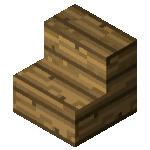
\includegraphics[width=4cm,height=\textheight,keepaspectratio,alt={Zeichnungstyp nodebox}]{bilder/drawtype_nodebox.png}
\caption{Zeichnungstyp nodebox}
\end{figure}

Mit Nodeboxen\index{nodebox@Nodebox} erstellst du Nodes, die nicht
würfelförmig sind, sondern aus beliebig vielen Quadern bestehen.

\begin{Shaded}
\begin{Highlighting}[]
\VariableTok{core}\OperatorTok{.}\NormalTok{register\_node}\OperatorTok{(}\StringTok{"stairs:stair\_stone"}\OperatorTok{,} \OperatorTok{\{}
    \VariableTok{drawtype} \OperatorTok{=} \StringTok{"nodebox"}\OperatorTok{,}
    \VariableTok{paramtype} \OperatorTok{=} \StringTok{"light"}\OperatorTok{,}
    \VariableTok{node\_box} \OperatorTok{=} \OperatorTok{\{}
        \FunctionTok{type} \OperatorTok{=} \StringTok{"fixed"}\OperatorTok{,}
        \VariableTok{fixed} \OperatorTok{=} \OperatorTok{\{}
            \OperatorTok{\{} \OperatorTok{{-}}\DecValTok{0.5}\OperatorTok{,} \OperatorTok{{-}}\DecValTok{0.5}\OperatorTok{,} \OperatorTok{{-}}\DecValTok{0.5}\OperatorTok{,} \DecValTok{0.5}\OperatorTok{,} \DecValTok{0}\OperatorTok{,} \DecValTok{0.5} \OperatorTok{\},}
            \OperatorTok{\{} \OperatorTok{{-}}\DecValTok{0.5}\OperatorTok{,} \DecValTok{0}\OperatorTok{,} \DecValTok{0}\OperatorTok{,} \DecValTok{0.5}\OperatorTok{,} \DecValTok{0.5}\OperatorTok{,} \DecValTok{0.5} \OperatorTok{\},}
        \OperatorTok{\},}
    \OperatorTok{\},}
\OperatorTok{\})}
\end{Highlighting}
\end{Shaded}

Der wichtigste Teil ist die Nodebox-Tabelle:

\begin{Shaded}
\begin{Highlighting}[]
\OperatorTok{\{{-}}\DecValTok{0.5}\OperatorTok{,} \OperatorTok{{-}}\DecValTok{0.5}\OperatorTok{,} \OperatorTok{{-}}\DecValTok{0.5}\OperatorTok{,}       \DecValTok{0.5}\OperatorTok{,}    \DecValTok{0}\OperatorTok{,}  \DecValTok{0.5}\OperatorTok{\},}
\OperatorTok{\{{-}}\DecValTok{0.5}\OperatorTok{,}    \DecValTok{0}\OperatorTok{,}    \DecValTok{0}\OperatorTok{,}       \DecValTok{0.5}\OperatorTok{,}  \DecValTok{0.5}\OperatorTok{,}  \DecValTok{0.5}\OperatorTok{\}}
\end{Highlighting}
\end{Shaded}

Jede Zeile ist ein Quader; zusammen ergeben sie einen einzigen Node. Die
ersten drei Zahlen sind die Koordinaten (von −0,5 bis einschließlich
0,5) der unteren, vorderen, linken Ecke, die letzten drei die der
gegenüberliegenden Ecke. Die Reihenfolge ist X, Y, Z, wobei Y nach oben
zeigt.

Mit dem NodeBoxEditor\footnote{\url{https://forum.luanti.org/viewtopic.php?f=14&t=2840}}
kannst du Nodeboxen erstellen, indem du die Kanten ziehst. Das ist
anschaulicher als die Arbeit von Hand.

\subsection{Nodeboxen für
Wandmontage}\label{nodeboxen-fuxfcr-wandmontage}

Manchmal braucht man unterschiedliche Nodeboxen, je nachdem, ob der Node
auf dem Boden, an der Wand oder an der Decke platziert wird, etwa bei
Fackeln.

\begin{Shaded}
\begin{Highlighting}[]
\VariableTok{core}\OperatorTok{.}\NormalTok{register\_node}\OperatorTok{(}\StringTok{"default:sign\_wall"}\OperatorTok{,} \OperatorTok{\{}
    \VariableTok{drawtype} \OperatorTok{=} \StringTok{"nodebox"}\OperatorTok{,}
    \VariableTok{node\_box} \OperatorTok{=} \OperatorTok{\{}
        \FunctionTok{type} \OperatorTok{=} \StringTok{"wallmounted"}\OperatorTok{,}

        \CommentTok{{-}{-} Decke}
        \VariableTok{wall\_top} \OperatorTok{=} \OperatorTok{\{}
            \OperatorTok{\{}
                \OperatorTok{{-}}\DecValTok{0.4375}\OperatorTok{,}
                \DecValTok{0.4375}\OperatorTok{,}
                \OperatorTok{{-}}\DecValTok{0.3125}\OperatorTok{,}
                \DecValTok{0.4375}\OperatorTok{,}
                \DecValTok{0.5}\OperatorTok{,}
                \DecValTok{0.3125}\OperatorTok{,}
            \OperatorTok{\},}
        \OperatorTok{\},}

        \CommentTok{{-}{-} Boden}
        \VariableTok{wall\_bottom} \OperatorTok{=} \OperatorTok{\{}
            \OperatorTok{\{}
                \OperatorTok{{-}}\DecValTok{0.4375}\OperatorTok{,}
                \OperatorTok{{-}}\DecValTok{0.5}\OperatorTok{,}
                \OperatorTok{{-}}\DecValTok{0.3125}\OperatorTok{,}
                \DecValTok{0.4375}\OperatorTok{,}
                \OperatorTok{{-}}\DecValTok{0.4375}\OperatorTok{,}
                \DecValTok{0.3125}\OperatorTok{,}
            \OperatorTok{\},}
        \OperatorTok{\},}

        \CommentTok{{-}{-} Wand}
        \VariableTok{wall\_side} \OperatorTok{=} \OperatorTok{\{}
            \OperatorTok{\{}
                \OperatorTok{{-}}\DecValTok{0.5}\OperatorTok{,}
                \OperatorTok{{-}}\DecValTok{0.3125}\OperatorTok{,}
                \OperatorTok{{-}}\DecValTok{0.4375}\OperatorTok{,}
                \OperatorTok{{-}}\DecValTok{0.4375}\OperatorTok{,}
                \DecValTok{0.3125}\OperatorTok{,}
                \DecValTok{0.4375}\OperatorTok{,}
            \OperatorTok{\},}
        \OperatorTok{\},}
    \OperatorTok{\},}
\OperatorTok{\})}
\end{Highlighting}
\end{Shaded}

\section{Mesh-Nodes}\label{mesh-nodes}

Nodeboxen sind zwar meist einfacher zu erstellen, bestehen aber nur aus
Quadern. Außerdem sind sie nicht optimiert: Innenflächen werden auch
dann gezeichnet, wenn sie vollständig verdeckt sind.

Eine Fläche (\emph{face}) ist eine ebene Oberfläche eines Meshs. Eine
Innenfläche entsteht, wenn sich die Flächen zweier Nodeboxen überlappen.
Teile des Modells sind dann unsichtbar, werden aber trotzdem gezeichnet.

So registrierst du einen Mesh-Node:

\begin{Shaded}
\begin{Highlighting}[]
\VariableTok{core}\OperatorTok{.}\NormalTok{register\_node}\OperatorTok{(}\StringTok{"mymod:meshy"}\OperatorTok{,} \OperatorTok{\{}
    \VariableTok{drawtype} \OperatorTok{=} \StringTok{"mesh"}\OperatorTok{,}

    \CommentTok{{-}{-} Enthält die Textur für jedes „Material“}
    \VariableTok{tiles} \OperatorTok{=} \OperatorTok{\{}
        \StringTok{"mymod\_meshy.png"}\OperatorTok{,}
    \OperatorTok{\},}

    \CommentTok{{-}{-} Pfad zum Mesh}
    \VariableTok{mesh} \OperatorTok{=} \StringTok{"mymod\_meshy.b3d"}\OperatorTok{,}
\OperatorTok{\})}
\end{Highlighting}
\end{Shaded}

Achte darauf, dass das Mesh\index{mesh@Mesh} in einem Verzeichnis
\texttt{models} liegt. Meist gehört es in den Ordner deines eigenen
Mods; du kannst aber auch ein Mesh aus einem anderen Mod verwenden, von
dem deiner abhängt. Ein Mod, der weitere Möbel hinzufügt, kann zum
Beispiel die Modelle eines grundlegenden Möbel-Mods mitnutzen.

\section{Signlike-Nodes}\label{signlike-nodes}

Signlike-Nodes sind flache Nodes, die an den Seiten anderer Nodes
angebracht werden. Trotz des Namens verwenden Schilder meist nicht
\texttt{signlike}, sondern \texttt{nodebox}, um einen 3D-Effekt zu
erzielen. Leitern dagegen nutzen häufig \texttt{signlike}.

\begin{Shaded}
\begin{Highlighting}[]
\VariableTok{core}\OperatorTok{.}\NormalTok{register\_node}\OperatorTok{(}\StringTok{"default:ladder\_wood"}\OperatorTok{,} \OperatorTok{\{}
    \VariableTok{drawtype} \OperatorTok{=} \StringTok{"signlike"}\OperatorTok{,}

    \VariableTok{tiles} \OperatorTok{=} \OperatorTok{\{} \StringTok{"default\_ladder\_wood.png"} \OperatorTok{\},}

    \CommentTok{{-}{-} Erforderlich: Drehung in param2 speichern}
    \VariableTok{paramtype2} \OperatorTok{=} \StringTok{"wallmounted"}\OperatorTok{,}

    \VariableTok{selection\_box} \OperatorTok{=} \OperatorTok{\{}
        \FunctionTok{type} \OperatorTok{=} \StringTok{"wallmounted"}\OperatorTok{,}
    \OperatorTok{\},}
\OperatorTok{\})}
\end{Highlighting}
\end{Shaded}

\section{Plantlike-Nodes}\label{plantlike-nodes}

\begin{figure}
\centering
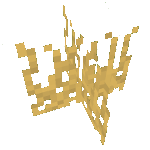
\includegraphics[width=4cm,height=\textheight,keepaspectratio,alt={Zeichnungstyp plantlike}]{bilder/drawtype_plantlike.png}
\caption{Zeichnungstyp plantlike}
\end{figure}

Plantlike-Nodes zeichnen ihre Textur in einem X-förmigen Muster.

\begin{Shaded}
\begin{Highlighting}[]
\VariableTok{core}\OperatorTok{.}\NormalTok{register\_node}\OperatorTok{(}\StringTok{"default:papyrus"}\OperatorTok{,} \OperatorTok{\{}
    \VariableTok{drawtype} \OperatorTok{=} \StringTok{"plantlike"}\OperatorTok{,}

    \CommentTok{{-}{-} Nur eine Textur}
    \VariableTok{tiles} \OperatorTok{=} \OperatorTok{\{} \StringTok{"default\_papyrus.png"} \OperatorTok{\},}

    \VariableTok{selection\_box} \OperatorTok{=} \OperatorTok{\{}
        \FunctionTok{type} \OperatorTok{=} \StringTok{"fixed"}\OperatorTok{,}
        \VariableTok{fixed} \OperatorTok{=} \OperatorTok{\{}
            \OperatorTok{{-}}\DecValTok{6} \OperatorTok{/} \DecValTok{16}\OperatorTok{,}
            \OperatorTok{{-}}\DecValTok{0.5}\OperatorTok{,}
            \OperatorTok{{-}}\DecValTok{6} \OperatorTok{/} \DecValTok{16}\OperatorTok{,}
            \DecValTok{6} \OperatorTok{/} \DecValTok{16}\OperatorTok{,}
            \DecValTok{0.5}\OperatorTok{,}
            \DecValTok{6} \OperatorTok{/} \DecValTok{16}\OperatorTok{,}
        \OperatorTok{\},}
    \OperatorTok{\},}
\OperatorTok{\})}
\end{Highlighting}
\end{Shaded}

\section{Firelike-Nodes}\label{firelike-nodes}

\texttt{firelike} ähnelt \texttt{plantlike}, ist aber so gestaltet, dass
es an Wänden und Decken „haftet``.

\begin{figure}
\centering
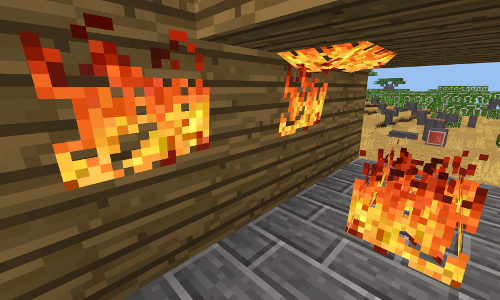
\includegraphics[width=7cm,height=\textheight,keepaspectratio,alt={Firelike-Nodes}]{bilder/drawtype_firelike.png}
\caption{Firelike-Nodes}
\end{figure}

\begin{Shaded}
\begin{Highlighting}[]
\VariableTok{core}\OperatorTok{.}\NormalTok{register\_node}\OperatorTok{(}\StringTok{"mymod:clinger"}\OperatorTok{,} \OperatorTok{\{}
    \VariableTok{drawtype} \OperatorTok{=} \StringTok{"firelike"}\OperatorTok{,}

    \CommentTok{{-}{-} Nur eine Textur}
    \VariableTok{tiles} \OperatorTok{=} \OperatorTok{\{} \StringTok{"mymod\_clinger.png"} \OperatorTok{\},}
\OperatorTok{\})}
\end{Highlighting}
\end{Shaded}

\section{Weitere Zeichnungstypen}\label{weitere-zeichnungstypen}

Die Liste ist nicht vollständig; es gibt noch weitere Typen, darunter:

\begin{itemize}
\tightlist
\item
  \texttt{fencelike}
\item
  \texttt{plantlike\_\allowbreak{}rooted} -- für Unterwasserpflanzen
\item
  \texttt{raillike} -- für Schienen
\item
  \texttt{torchlike} -- für 2D-Nodes an Wand, Boden oder Decke. Die
  Fackeln in Minetest Game verwenden allerdings Mesh-Nodes mit drei
  getrennten Definitionen (\texttt{default:torch},
  \texttt{default:torch\_\allowbreak{}wall} und
  \texttt{default:torch\_\allowbreak{}ceiling}).
\end{itemize}

Die vollständige Liste findest du wie immer in der
Lua-API-Dokumentation\footnote{\url{https://api.luanti.org/nodes/\#node-drawtypes}}.
